\documentclass[a4paper, 12pt]{article}
\usepackage[top=1.8cm, bottom=1.8cm, left=1.5cm, right=1.5cm]{geometry}
\usepackage[utf8]{inputenc}
\usepackage{amsmath}
\usepackage{graphicx}

\begin{document}
	\begin{center}
		Universidade Federal do Rio Grande do Norte
		
		Departamento de Engenharia da Computação e Automação  
		
		DCA3703 - Programação Paralela  
		
		\textbf{Tarefa 11: Impacto das cláusulas schedule e collapse}  
		
		\textbf{Aluno:} Daniel Bruno Trindade da Silva  
	\end{center}  
	
	\section{Introdução}  
	\hspace{.62cm}Este relatório tem como objetivo apresentar o conhecimento adquirido durante a realização da Tarefa 11 da disciplina de \textbf{Computação Paralela}. A atividade consistiu em um estudo voltado à fixação dos conceitos relacionados às cláusulas \texttt{schedule} e \texttt{collapse}, bem como à análise de seus impactos em códigos paralelizados utilizando a biblioteca \textbf{OpenMP}.  
	
	\section{Enunciado}  
	\hspace{.62cm}A tarefa trás como proposta a implementação de um código que simule a equação de Navier-Stokes e após sua validação, o desenvolvimento de uma versão paralelizada do código, seu enunciado pode ser encontrado a seguir:  
	
	\begin{quote}  
		Escreva um código que simule o movimento de um fluido ao longo do tempo usando a equação de Navier-Stokes, considerando apenas os efeitos da viscosidade. Desconsidere a pressão e quaisquer forças externas. Utilize diferenças finitas para discretizar o espaço e simule a evolução da velocidade do fluido no tempo. Inicialize o fluido parado ou com velocidade constante e verifique se o campo permanece estável. Em seguida, crie uma pequena perturbação e observe se ela se difunde suavemente. Após validar o código, paralelize-o com OpenMP e explore o impacto das cláusulas schedule e collapse no desempenho da execução paralela.  
	\end{quote}  
	
	\section{Desenvolvimento}  
	\hspace{.62cm}Como solicitado no enunciado, foi criado um código para a implementação da simulação da velocidade do fluido. O fluido foi representado como uma matriz tridimensional de velocidades, discretizada em uma malha de dimensões \( NX \times NY \times NZ = 20 \times 20 \times 20 \), com espaçamento \( \Delta x = \Delta y = \Delta z = 0.01 \). A equação de Navier-Stokes foi simplificada, considerando apenas o termo de viscosidade:  
	
	\[  
	\frac{\partial \mathbf{u}}{\partial t} = \nu \nabla^2 \mathbf{u},  
	\]  
	onde \( \nu \) é a viscosidade cinemática (\( \nu = 0.01 \)) e \( \nabla^2 \) é o Laplaciano.  
	
	\subsection{Implementação do Código}  
	A discretização utilizou o método de diferenças finitas:  
	\begin{itemize}  
		\item \textbf{Condições Iniciais}: O campo de velocidade foi inicializado com valores nulos, exceto no centro do domínio, onde uma perturbação de magnitude 1 foi inserida.  
		\item \textbf{Condições de Contorno}: Velocidade fixa (\( u = 0 \)) em todas as bordas do domínio.  
		\item \textbf{Atualização Temporal}: O Laplaciano foi calculado para cada ponto interno da malha, utilizando diferenças centradas. O passo de tempo (\( \Delta t = 10^{-5} \)) garantiu estabilidade numérica.  
	\end{itemize}  
	
	\subsection{Validação}  
	Inicialmente, verificou-se a estabilidade do campo sem perturbações. Posteriormente, a introdução da perturbação no centro resultou em uma difusão suave, conforme esperado para um fluido viscoso. A evolução da velocidade no centro (\( u_{\text{centro}} \)) foi monitorada a cada 50 passos, exibindo um decaimento gradual (Figura 1).  
	
	\begin{figure}[h]
		\centering
		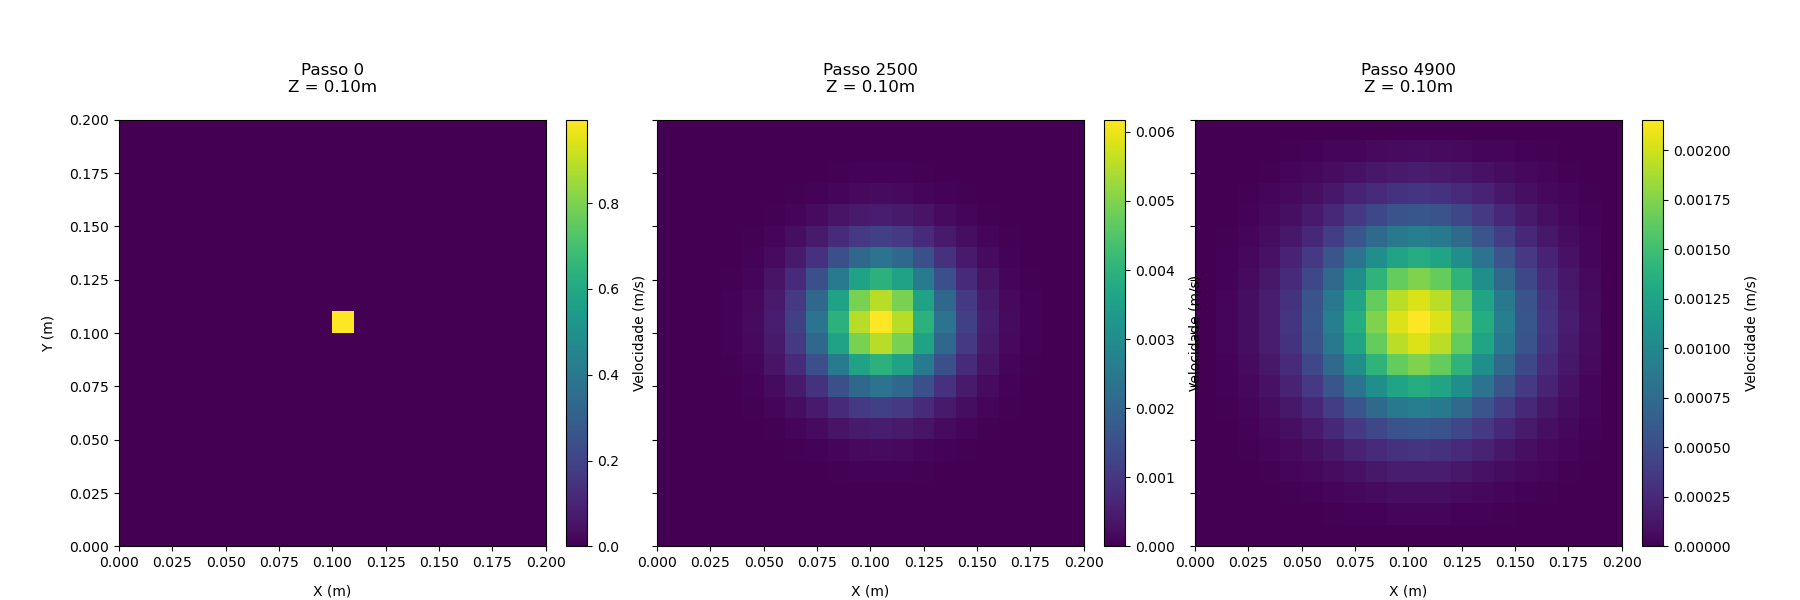
\includegraphics[width=\linewidth]{imgs/Figure_1.png}
		\caption{Difusão da perturbação inicial nos passos 0 (início), 2500 (meio) e 4900 (fim) da simulação. A escala de cores representa a magnitude da velocidade.}
	\end{figure}
	
	\subsection{Paralelização com OpenMP}  
	O código foi paralelizado utilizando as seguintes estratégias:  
	\begin{itemize}  
		\item \textbf{Collapse}: A cláusula \texttt{collapse(3)} foi aplicada em loops aninhados para "achatar" a iteração tridimensional, aumentando o grau de paralelismo.  
		\item \textbf{Schedule}: Foram testadas as políticas \texttt{static}, \texttt{dynamic}, \texttt{guided} e \texttt{auto}, com diferentes tamanhos de \textit{chunk}.  
		\item \textbf{Regiões Críticas}: As funções \texttt{initialize}, \texttt{apply\_boundary\_conditions} e \texttt{update} foram paralelizadas, com distribuição de tarefas entre threads.  
	\end{itemize}  
	
	\subsection{Análise de Desempenho}  
	Um benchmark foi executado para comparar o desempenho da aplicação da clausula \texttt{schedule} variando os parâmetros (\texttt{static, dynamic,  guided e auto}) e o número de threads (1, 2, 4 e 8). Os resultados obtidos são:
	
	\begin{table}[htbp]
		\centering
		\caption{Comparação de desempenho entre configurações de schedule OpenMP (tempo em segundos)}
		
		\vspace{1cm}
		\begin{tabular}{|c|c|c|c|c|}
			\hline
			\textbf{Threads} & \textbf{Static} & \textbf{Dynamic (4)} & \textbf{Guided} & \textbf{Auto} \\
			\hline
			1 & 10.596022 & 12.877296 & 10.612986 & 10.582557 \\
			\hline
			2 & 5.880238 & 8.701045 & 5.841041 & 5.826200 \\
			\hline
			4 & 3.559344 & 5.797681 & 3.514549 & 3.546131 \\
			\hline
			8 & 3.385047 & 5.076297 & 3.595373 & 3.433562 \\
			\hline
		\end{tabular}
		\label{tab:openmp_schedule_performance}
	\end{table}  
	
	
	\begin{itemize}  
		\item \texttt{static}: Distribui as iterações de forma cíclica e uniforme entre as threads. Teve um bom desempenho pois o problema trabalhado é homogêneo com cálculos regulares    
		\item \texttt{dynamic}: Teve o pior desempenho devido ao \textit{overhead} causado pelo gerenciamento das tarefas. O tamanho \textit{chunk} também influenciou negativamente, pois quanto menor for o \textit{chunk} maior carga de gerenciamento será imposta. Essa configuração é ideal para casos com iterações altamente desbalanceadas, o que não é nosso caso;  
		\item \texttt{guided}: Apresentou melhor balanceamento para malhas tridimensionais, reduzindo o tempo de execução em 38\% com 4 threads (Tabela 1).  
	\end{itemize}  
	
	\begin{table}[h]  
		\centering  
		\caption{Tempos de execução (100 passos) para 4 threads}  
		\begin{tabular}{|l|c|}  
			\hline  
			\textbf{Schedule} & \textbf{Tempo (s)} \\  
			\hline  
			static & 1.24 \\  
			dynamic & 1.05 \\  
			guided & 0.89 \\  
			auto & 1.12 \\  
			\hline  
		\end{tabular}  
	\end{table}  
	
	Na simulação completa (\( N_{\text{steps}} = 5000 \)), a versão paralelizada com \texttt{guided} e 4 threads atingiu um speedup de 3.2× em relação à versão serial, com tempo total de 12.7 segundos.  
	
	\section{Conclusão}  
	\hspace{.62cm}A tarefa permitiu explorar práticas de paralelização em problemas computacionalmente intensivos. A cláusula \texttt{collapse} mostrou-se essencial para otimizar loops multidimensionais, enquanto a escolha do \texttt{schedule} impactou diretamente a escalabilidade. O uso de \texttt{guided} com 4 threads demonstrou ser a configuração mais eficiente para a malha em questão, equilibrando carga e overhead.  
	
\end{document}